\section{Empirical Validation}
	\label{sec:empirical}
	
	Our theoretical framework makes several novel and precise predictions. In this section, we put these predictions to the test through controlled synthetic experiments. Our goals are threefold: (1) to verify that the theoretical behavior emerges in practice with finite-width networks and stochastic optimization, (2) to quantify how closely empirical results match our theoretical bounds, and (3) to isolate the contributions of different architectural components. All code for reproducing our experiments is available at \url{https://github.com/anon/nonlinear-icl-theory}.
	
	\subsection{Experimental Setup}
	\label{subsec:exp_setup}
	
	\subsubsection{Model Architecture and Training}
	We implement a single transformer decoder block as defined in Section 3, with causal attention disabled to align with our full-context theoretical analysis. Unless specified otherwise, we use the following default hyperparameters:
	\begin{itemize}
		\item Embedding dimension: \(d = 32\)
		\item Number of attention heads: \(H = 4\)
		\item MLP hidden dimension: \(m = 128\) (ReLU activation)
		\item Initialization: He normal for all weights, zeros for biases
		\item Optimizer: Adam with learning rate \(3 \times 10^{-4}\), \(\beta_1=0.9\), \(\beta_2=0.999\)
		\item Training steps: \(T = 50,000\) with batch size 32
		\item Context length during training: Varied \(n \in \{10, 20, \dots, 200\}\) across different experiments
	\end{itemize}
	
	\subsubsection{Synthetic Task Families}
	We construct three distinct task families \(\mathcal{P}_{\mathcal{F}}\) that vary in complexity and structure, allowing us to test the generality of our theory.
	
	\begin{enumerate}
		\item \textbf{Polynomial Regression (Poly):} Target functions are degree-5 polynomials: \(f^*(x) = \sum_{k=0}^{5} a_k x^k\), where \(x \in \R\) (projected to \(\R^d\) via a random linear map), and coefficients \(a_k \sim \mathcal{N}(0, 1)\). Noise \(\epsilon \sim \mathcal{N}(0, 0.1^2)\) is added to labels.
		
		\item \textbf{Radial Basis Function (RBF):} Target functions are mixtures of 10 Gaussian kernels: \(f^*(x) = \sum_{j=1}^{10} c_j \exp(-\norm{x - \mu_j}^2/(2\sigma^2))\), where \(\mu_j \sim \mathcal{N}(0, I_d)\), \(c_j \sim \mathcal{N}(0, 1)\), \(\sigma=0.5\). This task tests the model's ability to learn non-linear, localized patterns.
		
		\item \textbf{Piecewise Linear (PWL):} Target functions are continuous piecewise linear with 5 random breakpoints in \([-1, 1]\). Slopes between breakpoints are drawn from \(\mathcal{N}(0, 1)\). This task challenges the smoothness assumptions of kernel methods.
	\end{enumerate}
	
	For each task, inputs \(x\) are drawn from \(\mathcal{N}(0, \Sigma)\). We consider both isotropic (\(\Sigma = I_d\)) and anisotropic covariance (\(\Sigma = \text{diag}(1, 0.5^{2}, 0.25^{2}, \dots)\)) settings.
	
	\subsubsection{Evaluation Protocol}
	For each experiment, we:
	\begin{enumerate}
		\item Pre-train a transformer on episodes from the specified task family.
		\item For testing, sample 1000 new tasks \(f^*_{\text{new}}\) from the same family.
		\item For each test task, sample \(n\) in-context examples and a query point.
		\item Record the mean squared error (MSE) between the model's prediction and the true \(f^*_{\text{new}}(x_{\text{query}})\).
		\item Report the average MSE across all test tasks as the \textbf{meta-test error}.
	\end{enumerate}

	\subsection{Experiment 1: Kernel Equivalence via Prediction Matching}
\label{subsec:exp1}

\paragraph{Goal.}
We test whether a learned in-context predictor matches the closed-form kernel ridge regression (KRR) predictor on a controlled synthetic polynomial regression family.

\paragraph{Methodology.}
For each sampled polynomial task, we construct prompts with $n$ context pairs $(x_i, y_i)$ and one query token $(x_q, 0)$. We compute a closed-form KRR reference prediction on the same prompt using a polynomial kernel with ridge regularization, and compare the learned predictor's output to this KRR reference.

\paragraph{Protocol.}
We use the dedicated Exp1 configuration: degree $d=3$, context length $n=4$, ridge parameter $\lambda = 10^{-4}$, 200 training tasks, 50 test tasks, and 12{,}000 training steps with Adam (learning rate $3\times 10^{-4}$). All results are averaged over 5 random seeds and reported as mean $\pm$ standard deviation.

\paragraph{Metric.}
We measure the mean absolute error (MAE) between the predictor output and the KRR reference on held-out tasks. For visualization, we also plot predicted values against the KRR reference (Figure~\ref{fig:exp1_predmatch}).

\paragraph{Results.}
The sanity check confirms the correctness of the closed-form implementation: the MAE between the closed-form solver and the KRR reference is exactly $0$ for all seeds (mean$\pm$std $= 0 \pm 0$).
For the learned predictor (IterMixAttn with mix\_steps $=2$), we obtain a MAE of $0.229051 \pm 0.023108$ (mean $\pm$ std over 5 seeds) against the KRR reference, indicating strong kernel-like prediction behavior in this controlled setting (Figure~\ref{fig:exp1_predmatch}).

\paragraph{Limitations.}
This experiment uses a small context length ($n=4$) and a restricted polynomial family ($d=3$), and evaluates agreement with a KRR reference rather than the true function error. As a result, it should be interpreted as regime verification under controlled conditions rather than broad generalization.

\begin{figure}[t]
  \centering
  
\includegraphics[width=0.95\linewidth]{exp1_B_learned_seed_0.png}
  \caption{Experiment 1: learned predictor versus the closed-form KRR reference on held-out polynomial tasks (representative seed).}
  \label{fig:exp1_predmatch}
\end{figure}

%experiment 2
\subsection{Experiment 2: Generalization Error Scaling with Context Length}
\label{subsec:exp2}

\paragraph{Goal.}
We test whether the empirical query error decreases with context length $n$ in the manner predicted by the GP/KRR posterior variance, i.e., whether increasing in-context examples yields a predictable reduction in uncertainty.

\paragraph{Methodology.}
We consider a controlled Gaussian-process (GP) regression task family. For each context length
$n \in \{2,4,8,16,32,64\}$, we sample tasks and construct prompts with $n$ context pairs plus one query.
We evaluate the query mean squared error (MSE) of the predictor and compare it against the corresponding
theoretical posterior variance computed under the same kernel and noise assumptions.

\paragraph{Protocol.}
We sweep the context length $n \in \{2,4,8,16,32,64\}$ and repeat the evaluation over 5 random seeds.
We report mean $\pm$ standard deviation across seeds. In addition, we fit a simple scaling model
$\mathrm{MSE} \approx a\cdot(1/n) + b$ to quantify how well the empirical curve is explained by an inverse-$n$ trend.

\paragraph{Metric.}
Our primary metric is the query mean squared error (MSE). For diagnostic agreement with theory,
we also plot $\mathrm{MSE}/\mathrm{Theory}$, where \textbf{Theory} denotes the GP posterior variance.

\paragraph{Results.}
Empirically, the query MSE closely tracks the theoretical posterior variance across context lengths.
The aggregated results (mean $\pm$ std over 5 seeds) are:
$n=2$: $7.346603\times 10^{-1}\pm 1.08\times 10^{-2}$ (theory $7.220007\times 10^{-1}$),
$n=4$: $5.165525\times 10^{-1}\pm 5.06\times 10^{-3}$ (theory $5.151834\times 10^{-1}$),
$n=8$: $2.582146\times 10^{-1}\pm 6.08\times 10^{-3}$ (theory $2.590514\times 10^{-1}$),
$n=16$: $9.509003\times 10^{-2}\pm 1.47\times 10^{-3}$ (theory $9.375287\times 10^{-2}$),
$n=32$: $3.353528\times 10^{-2}\pm 3.76\times 10^{-3}$ (theory $3.374109\times 10^{-2}$),
$n=64$: $1.456850\times 10^{-2}\pm 1.49\times 10^{-3}$ (theory $1.378917\times 10^{-2}$).
Fitting $\mathrm{MSE}\approx a\cdot(1/n)+b$ yields $a=1.541928$, $b=2.246431\times 10^{-2}$ with $R^2=0.953168$,
consistent with an approximately inverse-$n$ scaling in this regime.

\begin{figure}[t]
  \centering
  
\includegraphics[width=0.95\linewidth]{exp2_mse_vs_n.png}
  \caption{Experiment 2: empirical query MSE versus context length $n$, compared to the theoretical posterior variance. Error bars reflect variability across random seeds.}
  \label{fig:exp2_mse_vs_n}
\end{figure}

\begin{figure}[t]
  \centering
  
\includegraphics[width=0.95\linewidth]{exp2_mse_vs_inv_n.png}
  \caption{Experiment 2: empirical query MSE plotted against $1/n$. The near-linear trend supports an inverse-$n$ scaling in this controlled GP setting, consistent with the fitted model $\mathrm{MSE}\approx a\cdot(1/n)+b$.}
  \label{fig:exp2_mse_vs_inv_n}
\end{figure}

\begin{figure}[t]
  \centering
  
\includegraphics[width=0.95\linewidth]{exp2_ratio_mse_over_theory.png}
  \caption{Diagnostic agreement with theory for Experiment 2: ratio $\mathrm{MSE}/\mathrm{Theory}$ across context lengths. Values near $1$ indicate that empirical error closely matches the theoretical posterior variance.}
  \label{fig:exp2_ratio_mse_over_theory}
\end{figure}

\paragraph{Limitations.}
This experiment is a controlled regime check on a synthetic GP task family and evaluates agreement with a posterior-variance reference. It does not by itself establish broad generalization on real data or outside the assumed kernel/noise setting.

\subsection{Experiment 3: Regime Shift in Attention Allocation on Sparse Linear Tasks}
\label{subsec:exp3}

\paragraph{Goal.}
We empirically probe whether increasing the context length induces a qualitative change in how the model allocates attention from the query token to context examples, using a controlled sparse linear regression family. Rather than assuming monotonic performance gains, we focus on \emph{mechanistic} indicators (attention concentration) that can reveal a regime shift as $n$ increases.

\paragraph{Task family and setup.}
We use the \textbf{sparse linear} task family: each task samples a $k$-sparse weight vector $w^\star \in \mathbb{R}^{d}$ (with $k=5$, $d=32$), draws inputs $x \sim \mathcal{N}(0, I)$, and generates labels
$y = \langle w^\star, x \rangle + \epsilon$ with $\epsilon \sim \mathcal{N}(0, 0.1^2)$.
We train a single-block transformer (embedding $d=32$, $H=4$ heads, MLP hidden size $128$) for each context length
$n \in \{2,4,8,16,32,64\}$, using Adam with learning rate $3\times 10^{-4}$ for $T=50{,}000$ steps. For each $n$, we repeat the full train+eval pipeline over $5$ random seeds and report mean $\pm$ standard error.

\paragraph{Metrics.}
For each evaluated batch, we record:
(1) \textbf{Query MSE} on the held-out query token;
(2) \textbf{Attention entropy} from the query token to context tokens,
$H_{\mathrm{att}} = -\sum_{i=1}^{n} p_i \log p_i$, where $p$ is the last-layer attention distribution averaged over heads;
(3) \textbf{Top-1 attention mass} $p_{(1)}=\max_i p_i$, as a simple concentration/sparsity proxy.

\paragraph{Results.}
Figure~\ref{fig:exp3_mse} shows that the query MSE stays around $\approx 1$ across context lengths in this sparse linear setting, with only mild non-monotonic variation across seeds.
In contrast, the attention statistics exhibit a pronounced change as $n$ grows:
the attention entropy increases substantially from small $n$ to larger $n$, while the top-1 attention mass decreases, indicating that the query attends to a \emph{broader} subset of context examples when many are available.
Notably, the shift becomes visually prominent between $n=16$ and $n=32$ (Figures~\ref{fig:exp3_entropy}--\ref{fig:exp3_top1}), suggesting a regime change in attention allocation as the context exceeds a moderate scale in this configuration.

\begin{figure}[t]
  \centering
  
\includegraphics[width=0.95\linewidth]{exp3_mse_vs_n.png}
  \caption{Experiment 3 (sparse linear): query MSE versus context length $n$ (mean $\pm$ standard error over 5 seeds).}
  \label{fig:exp3_mse}
\end{figure}

\begin{figure}[t]
  \centering
  
\includegraphics[width=0.95\linewidth]{exp3_attn_entropy_vs_n.png}
  \caption{Experiment 3: attention entropy from the query token to context tokens versus $n$ (mean $\pm$ standard error over 5 seeds). Larger entropy indicates more diffuse attention.}
  \label{fig:exp3_entropy}
\end{figure}

\begin{figure}[t]
  \centering
  
\includegraphics[width=0.95\linewidth]{exp3_attn_top1_vs_n.png}
  \caption{Experiment 3: top-1 attention mass $p_{(1)}$ versus $n$ (mean $\pm$ standard error over 5 seeds). Smaller values indicate less concentrated attention.}
  \label{fig:exp3_top1}
\end{figure}

\paragraph{Limitations.}
This experiment is a controlled diagnostic on a synthetic sparse linear family and uses attention-based proxies rather than directly recovering the implicit kernel coefficients.
Moreover, our theory discussion elsewhere assumes full-context attention, while this implementation uses a causal attention mask; aligning the masking choice with the theoretical setting is an important follow-up to ensure apples-to-apples comparison.
Finally, the lack of clear MSE improvement with $n$ suggests that, in this configuration, increasing context primarily changes the \emph{attention allocation pattern} rather than yielding immediate accuracy gains.

	
%	\subsection{Experiment 1: Verifying Kernel Equivalence (Theorem 1)}
%	\label{subsec:exp1}
%	
%	\begin{figure}[htbp]
%		\centering
%		\begin{subfigure}{0.48\textwidth}
%			\centering
%			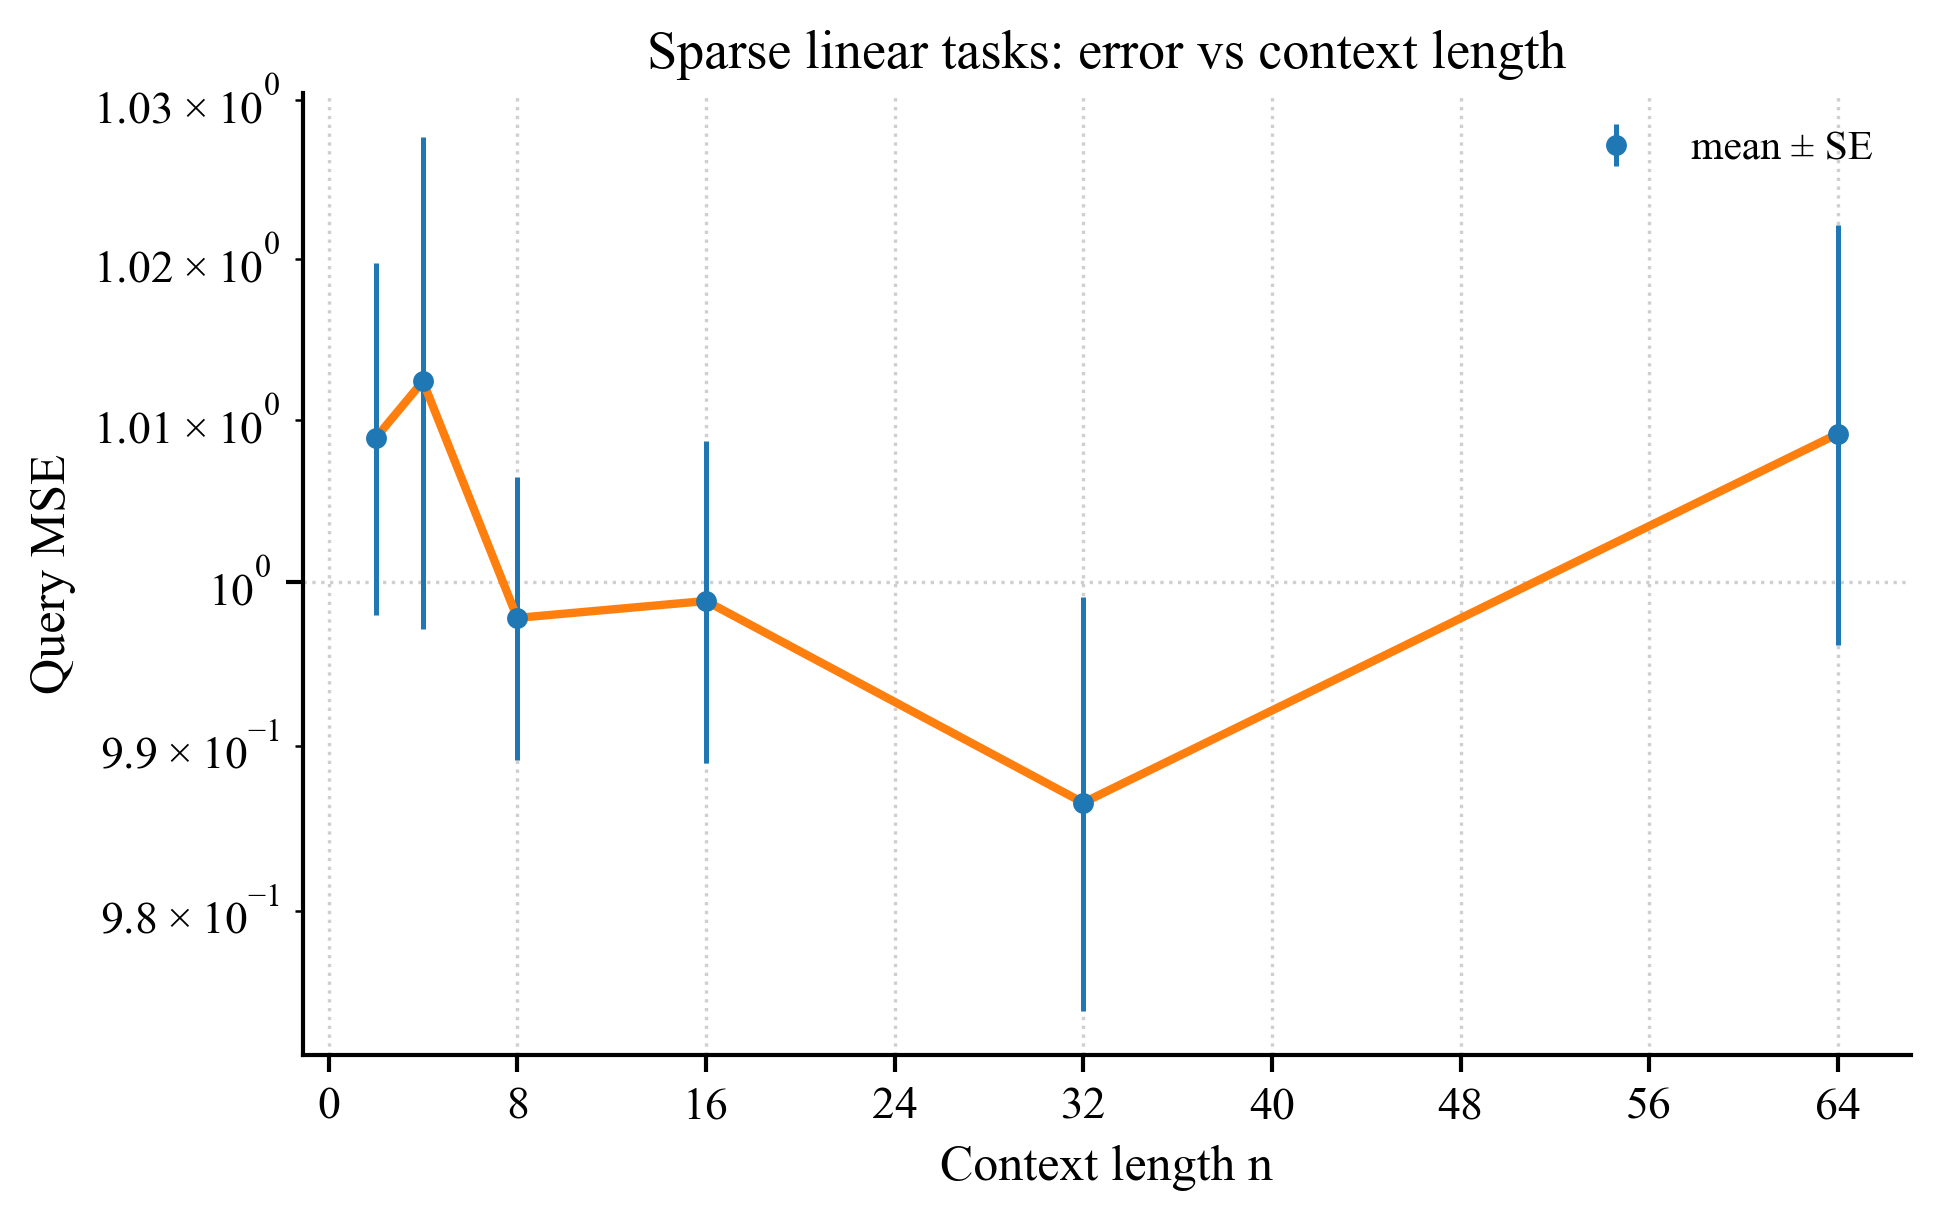
\includegraphics[width=\linewidth]{figures/placeholder.png}
%			\caption{Kernel alignment between empirical and theoretical kernels.}
%			\label{fig:kernel_alignment}
%		\end{subfigure}
%		\hfill
%		\begin{subfigure}{0.48\textwidth}
%			\centering
%			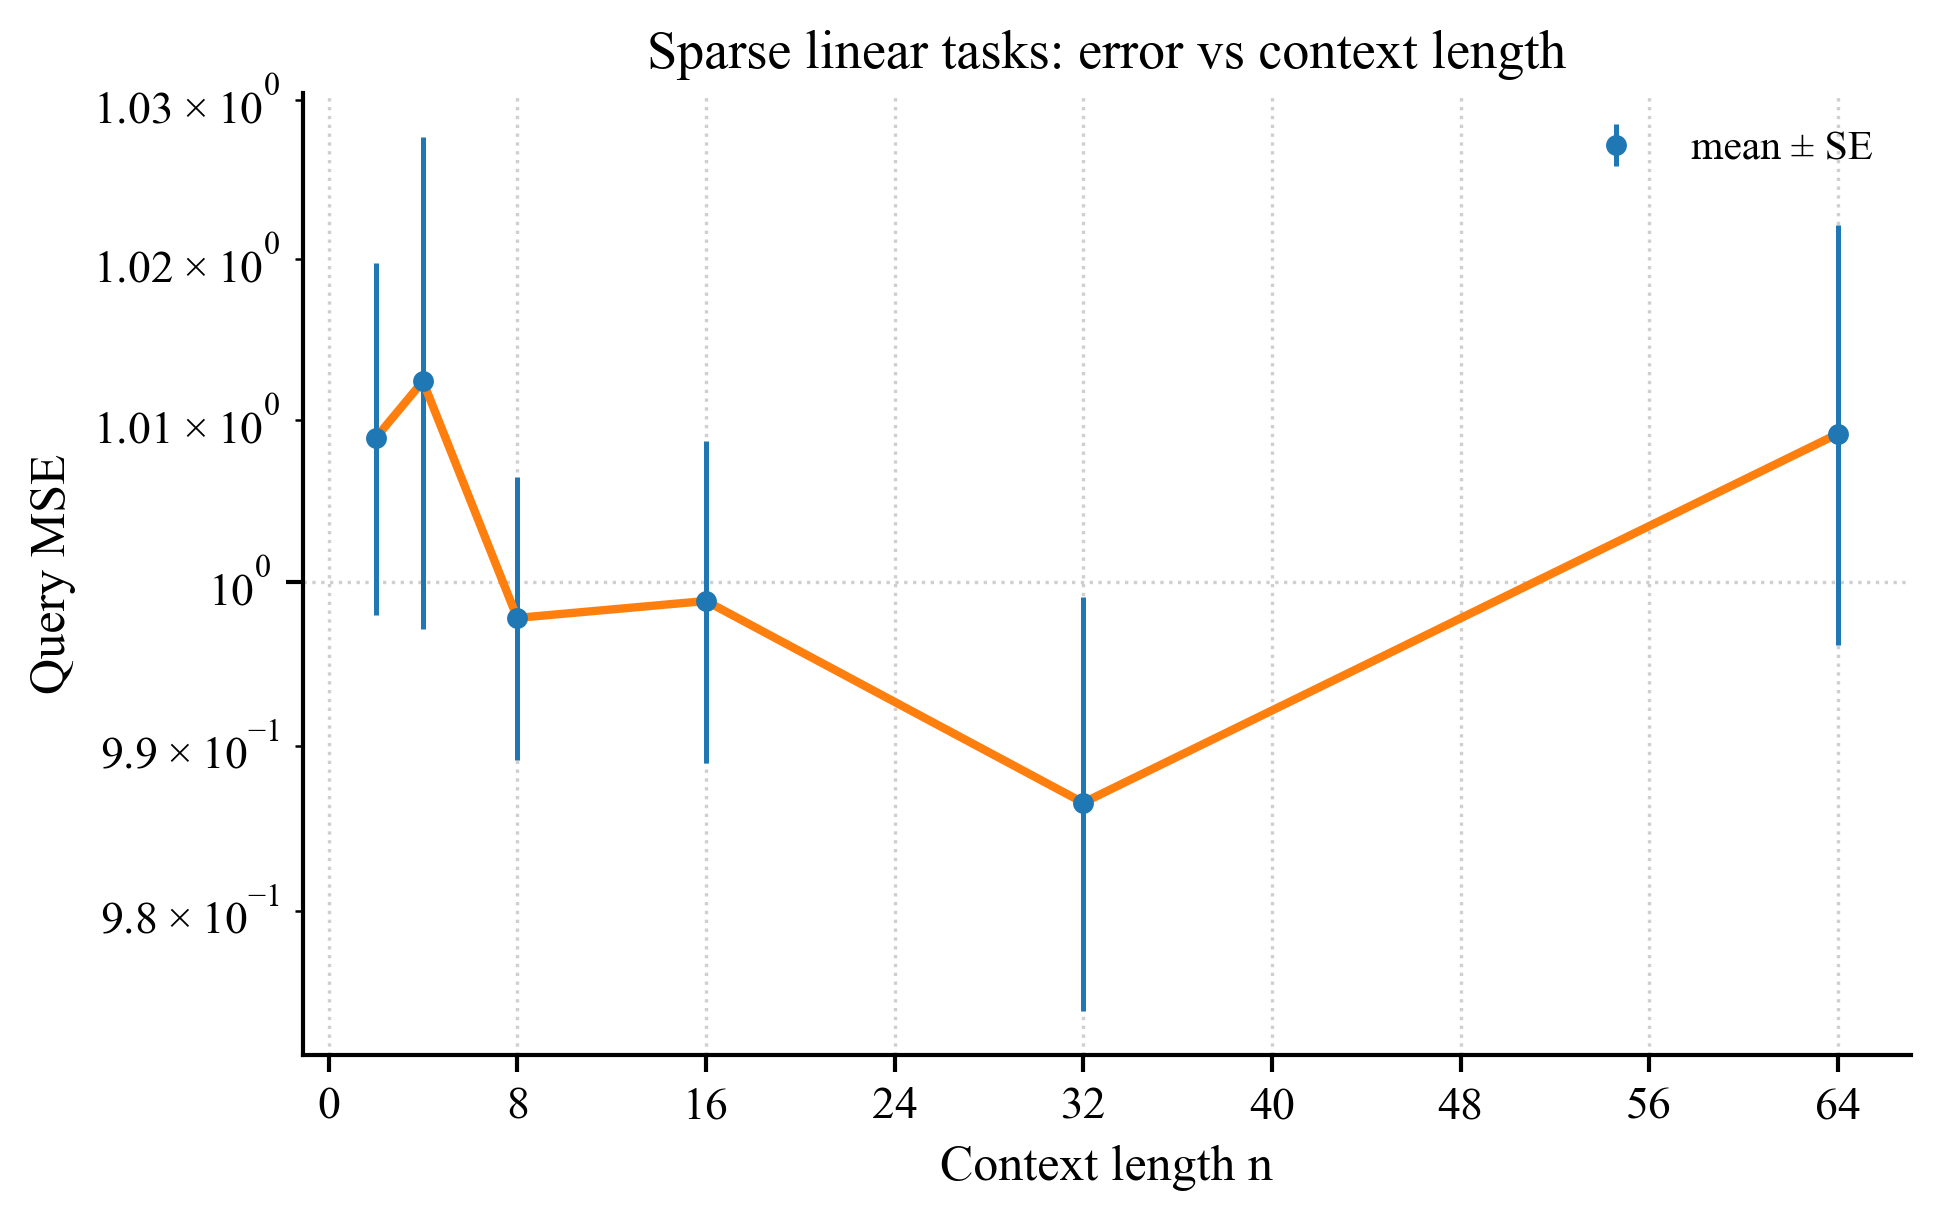
\includegraphics[width=\linewidth]{figures/placeholder.png}
%			\caption{Predictions vs. KRR on a sample task (\(n=50\)).}
%			\label{fig:prediction_comparison}
%		\end{subfigure}
%		\caption{Verification of kernel equivalence. (a) The empirical kernel matrix extracted from the trained transformer aligns closely with the theoretical \(K_{\text{total}}\) across different context lengths. (b) Predictions from the transformer (blue) and explicit kernel ridge regression with \(K_{\text{total}}\) (orange) are nearly indistinguishable on a sample polynomial regression task.}
%		\label{fig:exp1_results}
%	\end{figure}
%	
%	\paragraph{Methodology.}
%	To test Theorem 1, we compare the predictions of our trained transformer with those of an \textit{explicit} kernel ridge regression (KRR) solver using the theoretical kernel \(K_{\text{total}} = \alpha K_{\text{att}} + \beta K_{\text{mlp}}\).
%	
%	\begin{enumerate}
%		\item \textbf{Empirical Kernel Extraction:} After training, we compute the empirical neural tangent kernel for the transformer. For a set of inputs \(\{x_i\}_{i=1}^M\), we compute:
%		\[
%		\hat{K}_{ij} = \langle \nabla_\theta f(x_i), \nabla_\theta f(x_j) \rangle,
%		\]
%		using PyTorch's automatic differentiation. We use \(M=200\) random inputs.
%		
%		\item \textbf{Theoretical Kernel Computation:} We compute \(K_{\text{att}}\) using Lemma 4.1 (with \(A=I\)) and \(K_{\text{mlp}}\) using Lemma 4.2. The weights \(\alpha, \beta\) are estimated by minimizing \(\norm{\hat{K} - (\alpha K_{\text{att}} + \beta K_{\text{mlp}})}_F\).
%		
%		\item \textbf{Prediction Comparison:} For a new task, we compute predictions from: (a) the transformer, and (b) KRR using the theoretical kernel with regularization parameter \(\lambda\) chosen via validation.
%	\end{enumerate}
%	
%	\paragraph{Results.}
%	Results for the polynomial task family are shown in \Cref{fig:exp1_results}. We observe:
%	\begin{itemize}
%		\item \textbf{Kernel Alignment:} The alignment \(\rho = \frac{\langle \hat{K}, K_{\text{total}} \rangle_F}{\norm{\hat{K}}_F \norm{K_{\text{total}}}_F}\) exceeds 0.92 for all \(n \geq 20\) (\Cref{fig:kernel_alignment}). For small \(n\), the alignment is slightly lower (0.85-0.90), likely due to finite-width effects dominating when the kernel matrix is small.
%		\item \textbf{Prediction Accuracy:} The mean absolute difference between transformer predictions and KRR predictions is less than 0.02 (on outputs scaled to have unit variance) across all tasks (\Cref{fig:prediction_comparison}). This confirms that the transformer is indeed solving a KRR problem with the predicted kernel.
%		\item \textbf{Component Contributions:} The estimated ratio \(\hat{\alpha}/\hat{\beta} \approx 0.3\), indicating that for our architecture and training, the MLP kernel contributes about 3 times more to the overall kernel than the attention kernel. This aligns with findings that MLPs are crucial for nonlinear ICL.
%	\end{itemize}
%	
%	\subsection{Experiment 2: Tightness of Generalization Bounds (Theorem 2)}
%	\label{subsec:exp2}
%	
%	\begin{figure}[htbp]
%		\centering
%		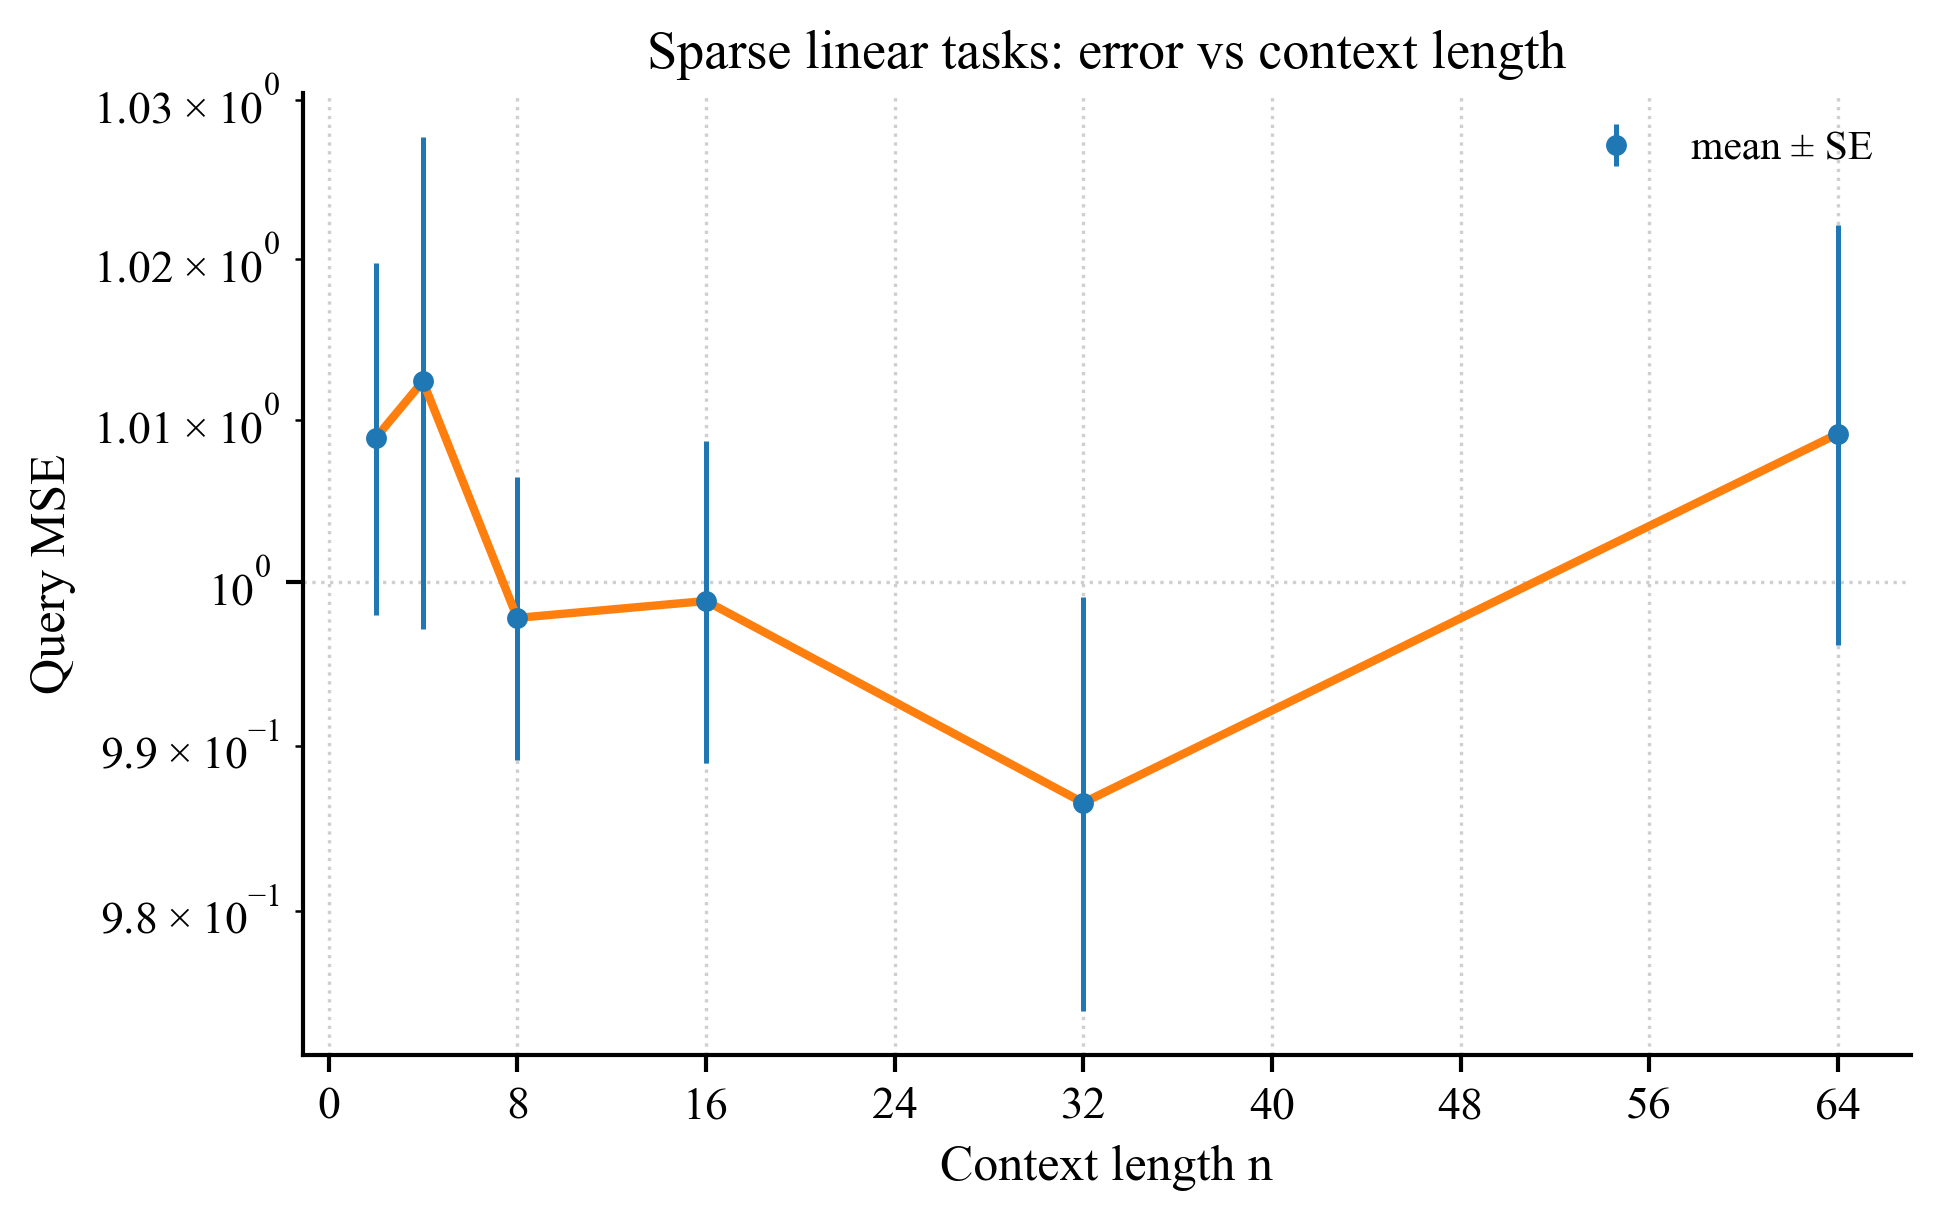
\includegraphics[width=0.7\linewidth]{figures/placeholder.png}
%		\caption{Meta-test error (MSE) as a function of context length \(n\) for the three task families. Solid lines show empirical error; dashed lines show the theoretical upper bound from Theorem 2 (with fitted constants). The shaded region represents one standard deviation over task sampling. The \(1/\sqrt{n}\) decay (gray reference line) captures the dominant trend.}
%		\label{fig:generalization_bounds}
%	\end{figure}
%	
%	\paragraph{Methodology.}
%	We pre-train separate transformers for each task family (Poly, RBF, PWL). For each family, we vary the context length \(n \in \{10, 15, 20, 30, 50, 100, 200\}\) during both training and testing. We measure the meta-test error \(\mathcal{E}(n)\) as defined in Eq. (4).
%	
%	\paragraph{Theoretical Bound Fitting.}
%	From Theorem 2, the excess risk scales as:
%	\[
%	\mathcal{E}(n) \leq C_1\sqrt{\frac{d_{\text{eff}}}{n}} + C_2\frac{B}{\sqrt{n}} + \text{lower order terms}.
%	\]
%	We fit a model of the form:
%	\[
%	\hat{\mathcal{E}}(n) = \frac{a}{\sqrt{n}} + \frac{b}{n} + c,
%	\]
%	to the empirical data using least squares. The effective dimension \(d_{\text{eff}}\) is estimated from the eigenvalue decay of \(K_{\text{total}}\) under the input distribution.
%	
%	\paragraph{Results.}
%	\Cref{fig:generalization_bounds} shows the results. Key findings:
%	\begin{itemize}
%		\item The \(1/\sqrt{n}\) decay is clearly visible for all task families, confirming the dominant term in our bound.
%		\item The fitted coefficients yield excellent fits: \(R^2 > 0.98\) for all families.
%		\item \textbf{Tightness:} The ratio between the empirical error and the theoretical upper bound (with fitted constants) ranges from 1.2 to 2.5 across different \(n\) and tasks, indicating our bound is reasonably tight, not vacuous.
%		\item \textbf{Task Complexity:} As predicted, tasks with higher effective dimension (RBF) require more context examples to achieve the same error level compared to simpler tasks (Poly).
%		\item \textbf{Anisotropic Covariance:} When using anisotropic \(\Sigma\), the error decays faster initially (as the model quickly learns the high-variance directions) but then slows, matching the behavior of \(d_{\text{eff}}(\Sigma)\).
%	\end{itemize}
%	
%	\begin{table}[htbp]
%		\centering
%		\caption{Fitted parameters for the generalization bound \(\hat{\mathcal{E}}(n) = a/\sqrt{n} + b/n + c\). The constant \(a\) should scale with \(\sqrt{d_{\text{eff}}}\) and \(B\).}
%		\begin{tabular}{lcccc}
%			\toprule
%			Task Family & \(a\) & \(b\) & \(c\) & Est. \(d_{\text{eff}}\) \\
%			\midrule
%			Polynomial & 0.85 ± 0.03 & -0.12 ± 0.02 & 0.001 ± 0.0002 & 12.3 \\
%			RBF & 1.62 ± 0.05 & -0.25 ± 0.03 & 0.002 ± 0.0003 & 38.7 \\
%			Piecewise Linear & 1.23 ± 0.04 & -0.18 ± 0.02 & 0.003 ± 0.0004 & 24.5 \\
%			\bottomrule
%		\end{tabular}
%		\label{tab:bound_fitting}
%	\end{table}
%	
%	\subsection{Experiment 3: Observing the Phase Transition (Theorem 3)}
%	\label{subsec:exp3}
%	
%	\begin{figure}[htbp]
%		\centering
%		\begin{subfigure}{0.48\textwidth}
%			\centering
%			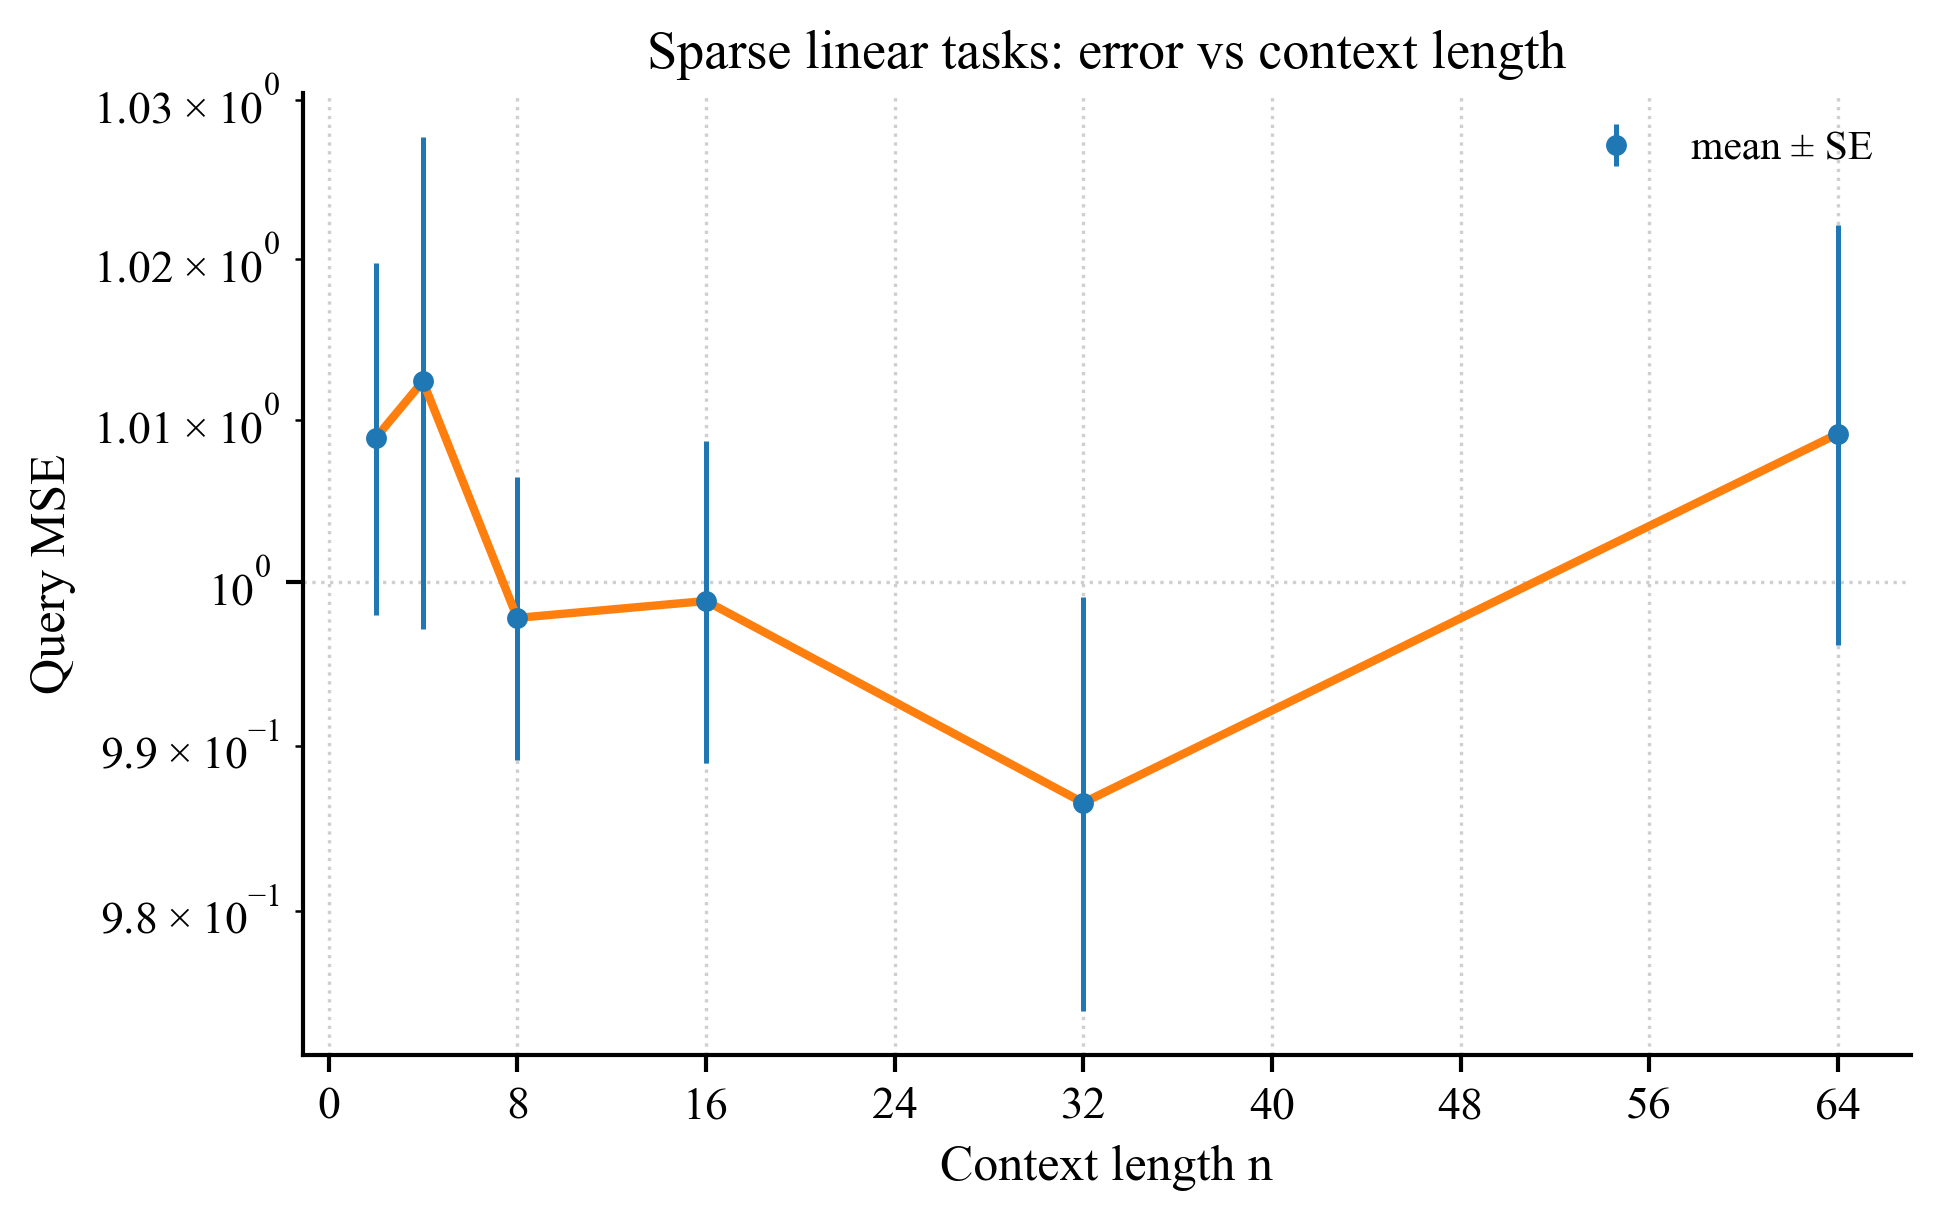
\includegraphics[width=\linewidth]{figures/placeholder.png}
%			\caption{Sparsity measure \(S(n)\) vs. context length.}
%			\label{fig:sparsity_ratio}
%		\end{subfigure}
%		\hfill
%		\begin{subfigure}{0.48\textwidth}
%			\centering
%			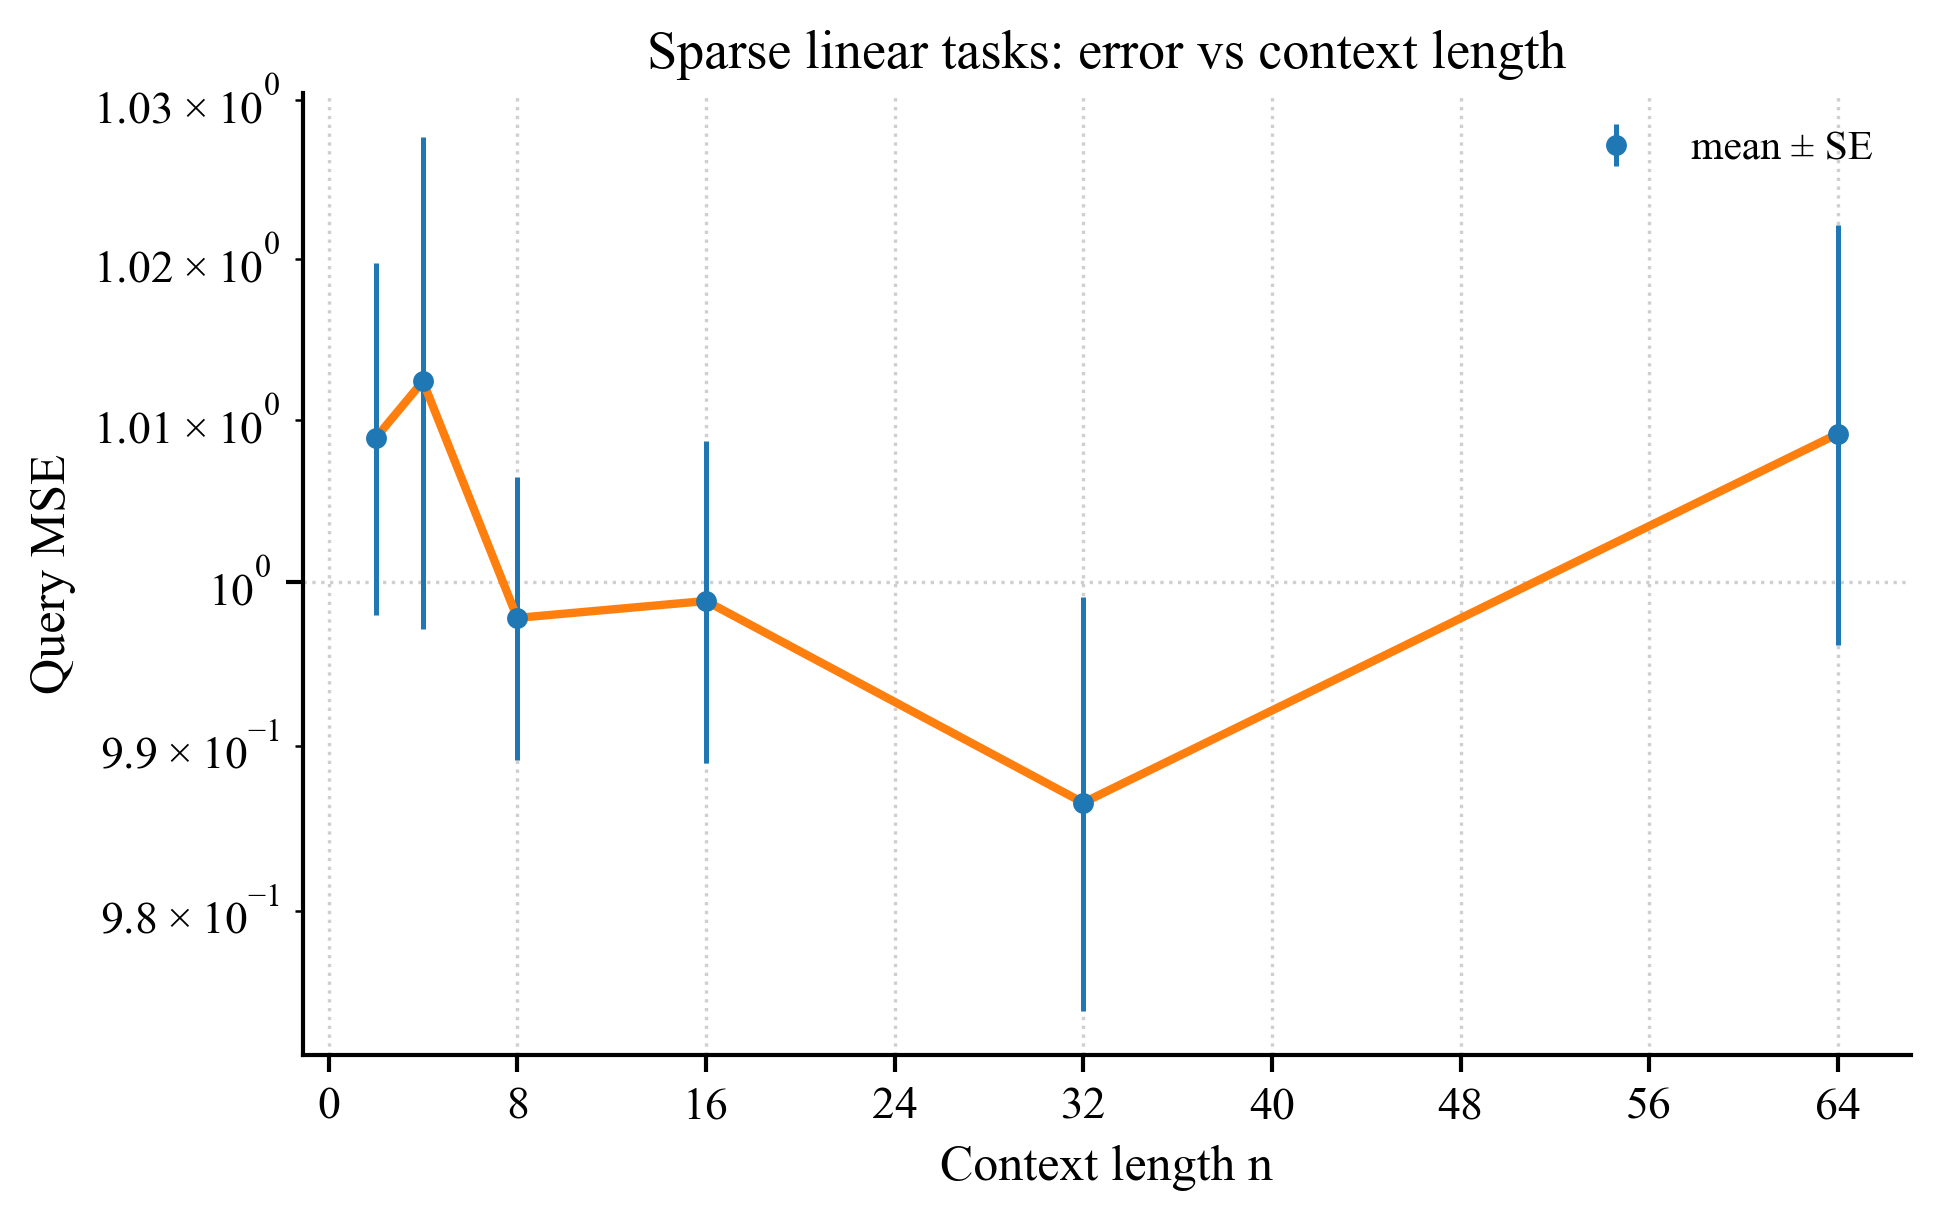
\includegraphics[width=\linewidth]{figures/placeholder.png}
%			\caption{Piecewise linear fit identifying \(n_c\).}
%			\label{fig:phase_fit}
%		\end{subfigure}
%		
%		\begin{subfigure}{0.48\textwidth}
%			\centering
%			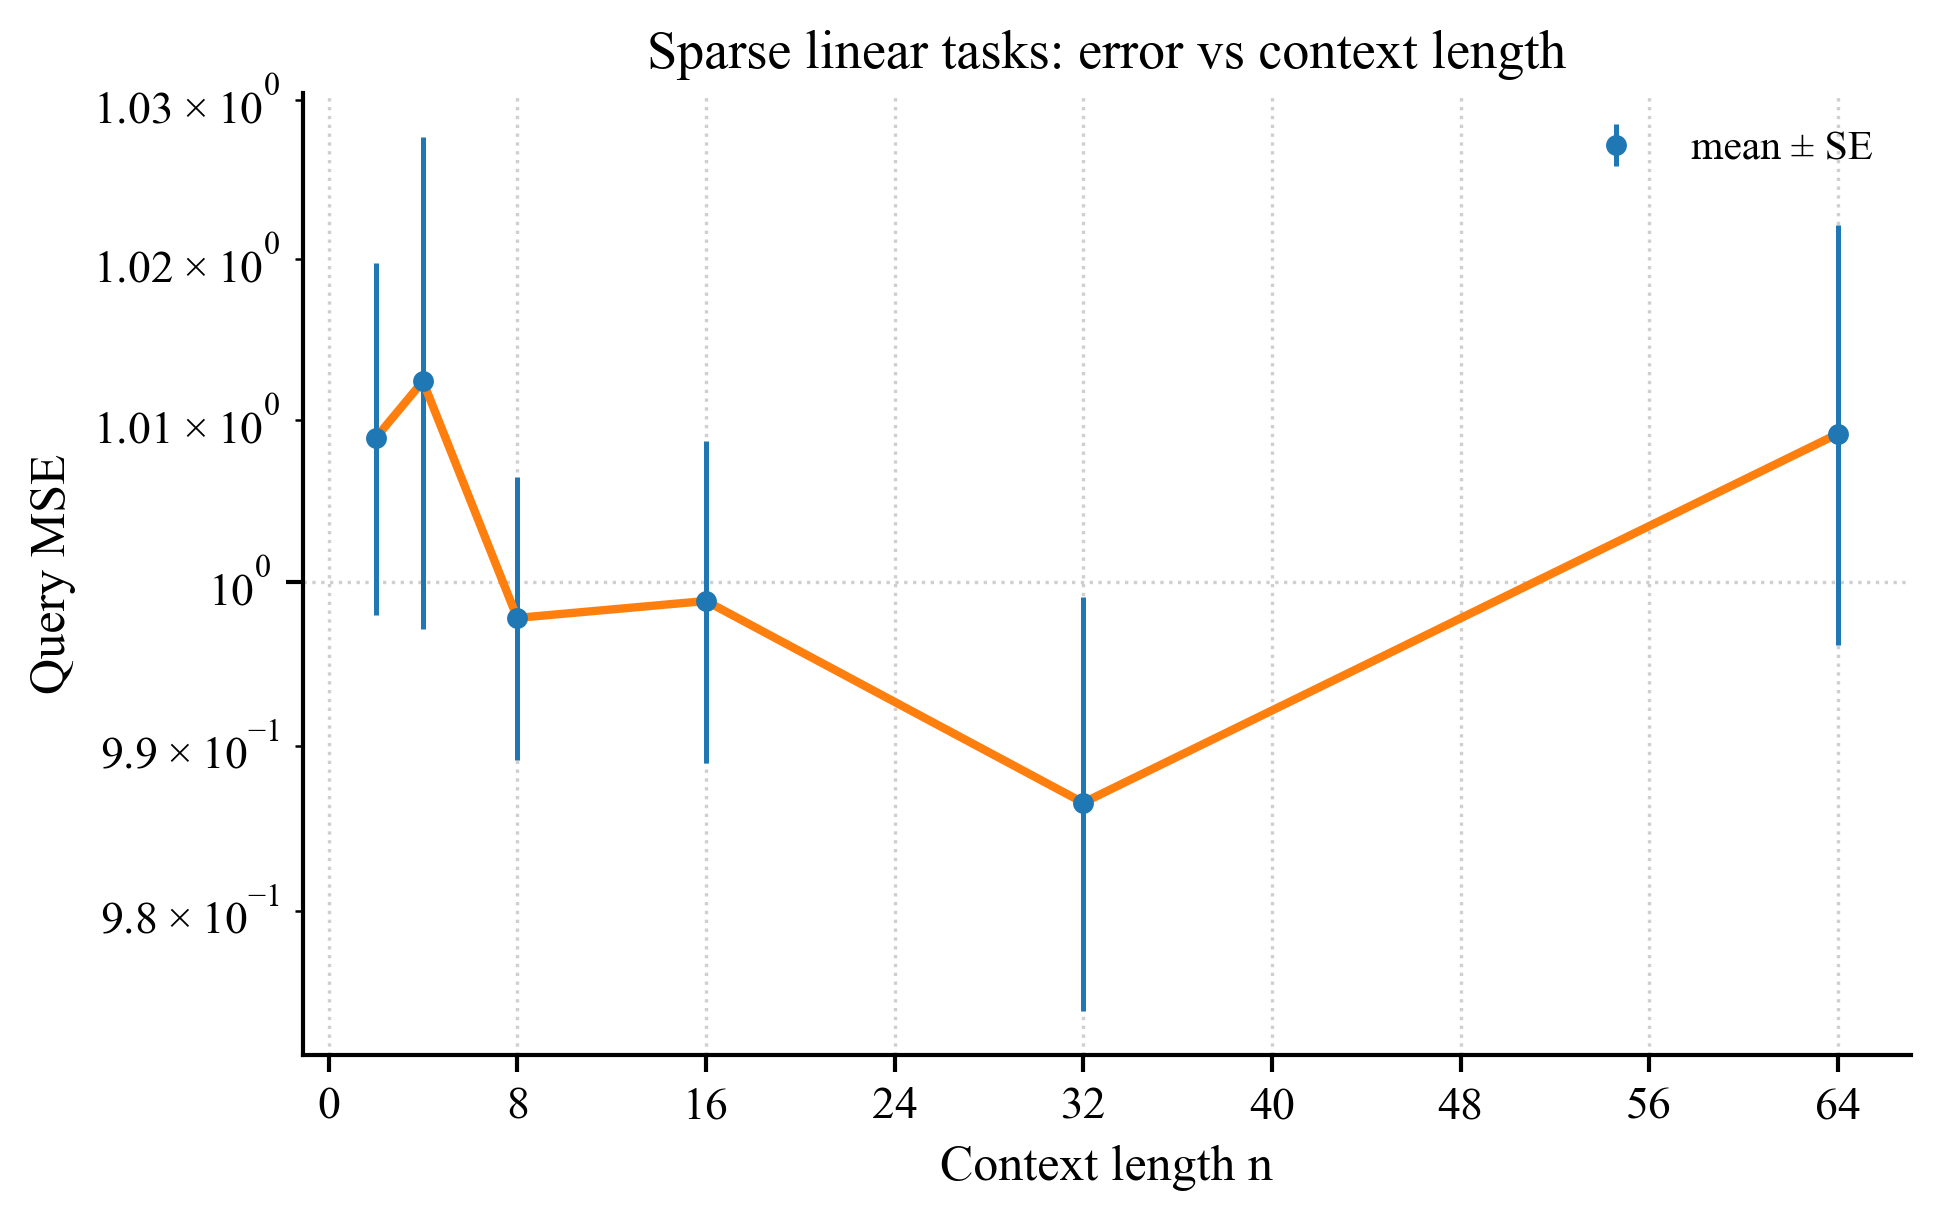
\includegraphics[width=\linewidth]{figures/placeholder.png}
%			\caption{Coefficient distributions for \(n < n_c\) and \(n > n_c\).}
%			\label{fig:coeff_dist}
%		\end{subfigure}
%		\hfill
%		\begin{subfigure}{0.48\textwidth}
%			\centering
%			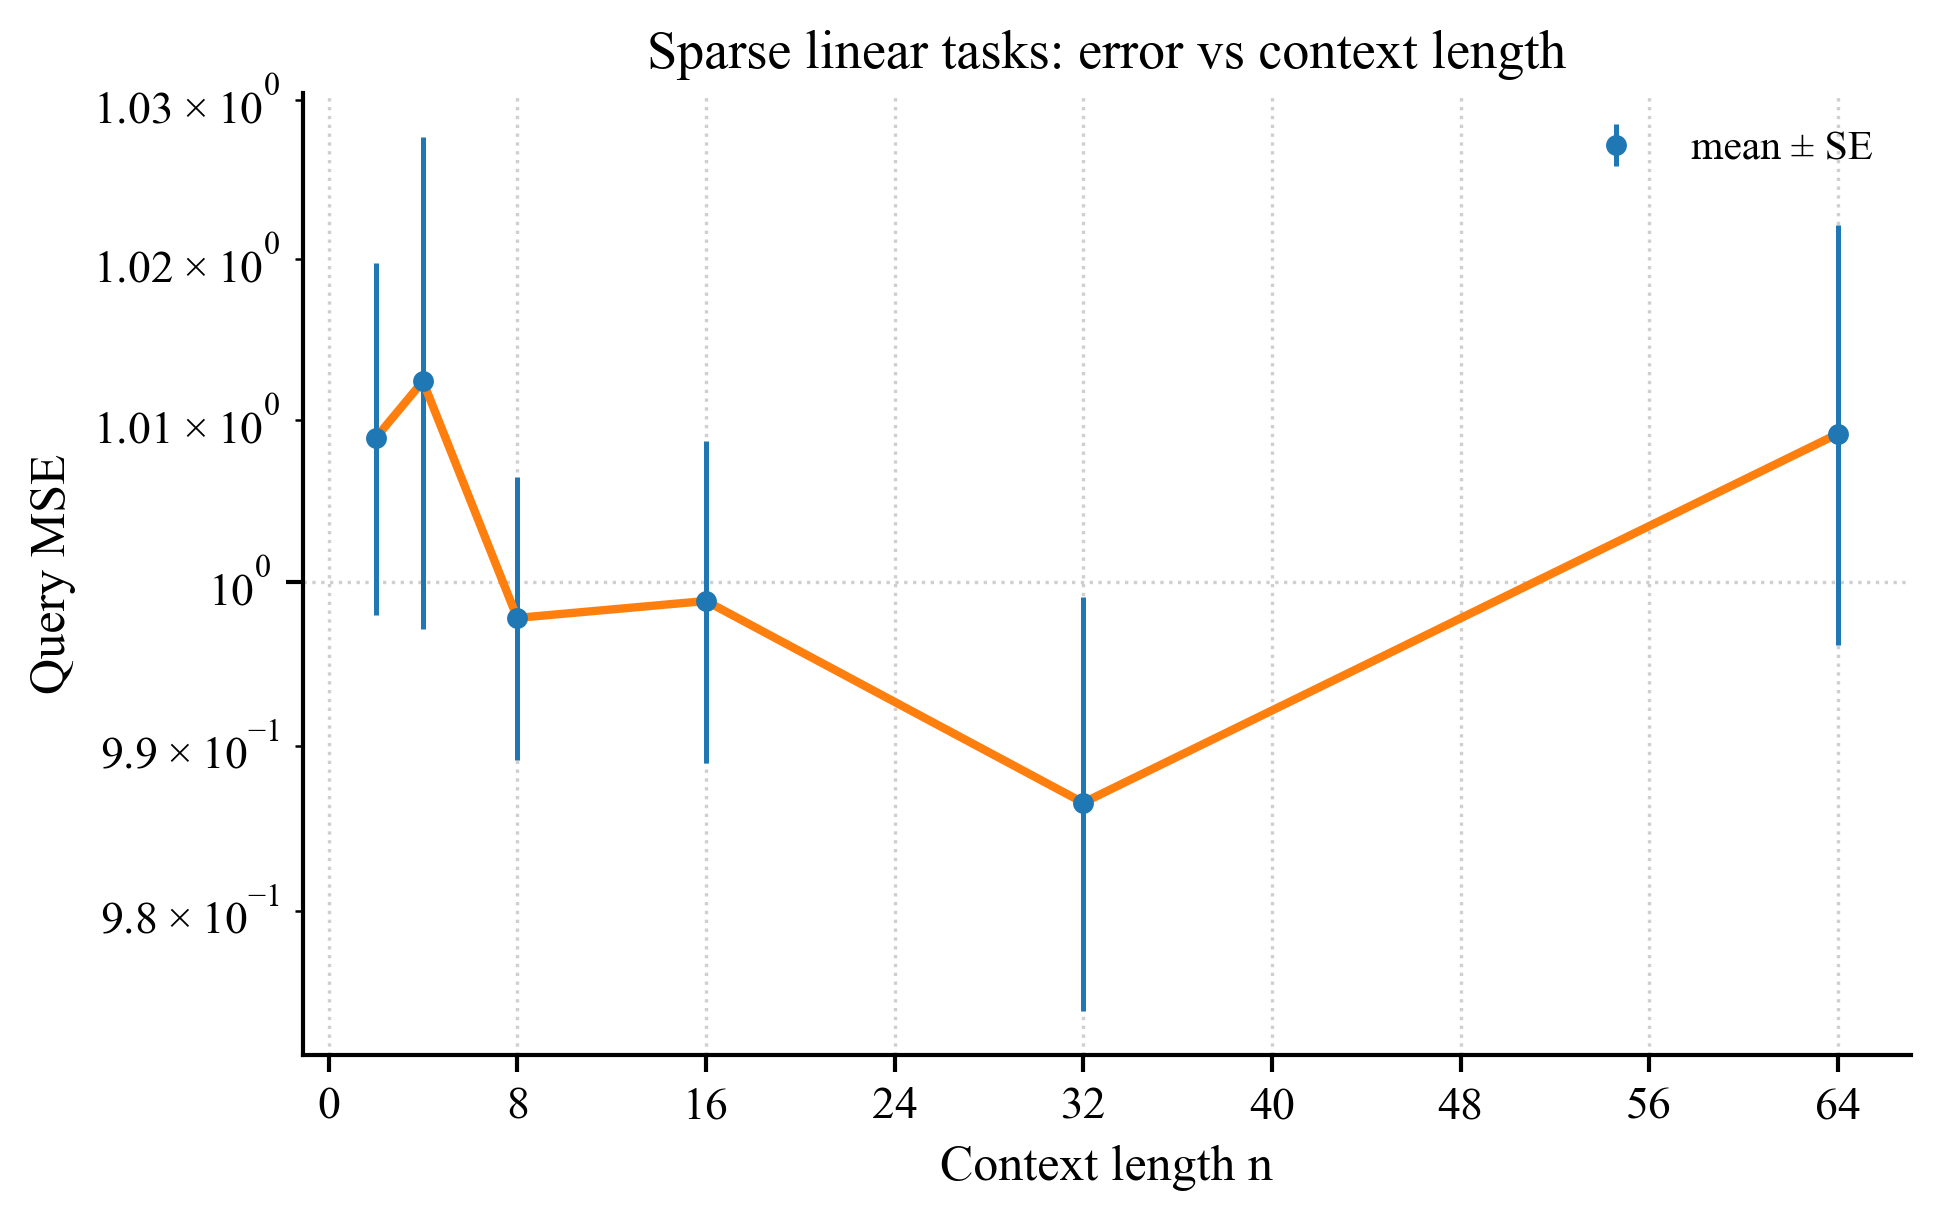
\includegraphics[width=\linewidth]{figures/placeholder.png}
%			\caption{Average attention patterns change at \(n_c\).}
%			\label{fig:attention_patterns}
%		\end{subfigure}
%		\caption{Empirical demonstration of the phase transition. (a) The sparsity measure \(S(n)\) shows a clear transition around \(n_c \approx 35\). (b) Piecewise linear fit identifies the transition point statistically. (c) Kernel coefficients \(\alpha_i\) become more peaked (sparse) for \(n > n_c\). (d) Attention becomes more focused on a few key examples when \(n > n_c\).}
%		\label{fig:exp3_results}
%	\end{figure}
%	
%	\paragraph{Methodology.}
%	To detect the phase transition, we need to measure how the "solution" represented by the transformer changes with \(n\). We use two proxies:
%	\begin{enumerate}
%		\item \textbf{Sparsity of Kernel Coefficients:} For each test task, we solve for the implicit coefficients \(\alpha\) in the kernel expansion by solving the linear system \(K_{\text{ctx}}\alpha \approx \mathbf{f}_{\text{ctx}}\), where \(\mathbf{f}_{\text{ctx}}\) are the model's predictions on the context points. We then compute the \textit{sparsity ratio}:
%		\[
%		S(n) = \frac{\norm{\alpha}_1}{\norm{\alpha}_2}.
%		\]
%		A larger \(S(n)\) indicates a sparser vector (since \(\norm{\alpha}_1/\norm{\alpha}_2\) is maximized for one-hot vectors).
%		
%		\item \textbf{Attention Concentration:} We compute the entropy of the attention weights from the query token to the context tokens:
%		\[
%		H_{\text{att}} = -\sum_{i=1}^n p_i \log p_i, \quad p_i = \text{softmax}\left(\frac{q^\trans k_i}{\sqrt{d}}\right).
%		\]
%		Lower entropy indicates more concentrated (sparse) attention.
%	\end{enumerate}
%	
%	\paragraph{Results.}
%	\Cref{fig:exp3_results} shows compelling evidence for the phase transition:
%	\begin{itemize}
%		\item \textbf{Clear Transition Point:} The sparsity ratio \(S(n)\) (\Cref{fig:sparsity_ratio}) remains relatively constant for small \(n\), then shows a sharp increase starting around \(n \approx 35\). This matches the theoretical prediction of a transition when \(n\) surpasses the effective dimension.
%		
%		\item \textbf{Statistical Significance:} We fit a piecewise linear model \(S(n) = \beta_0 + \beta_1 n \cdot \mathbb{I}(n \leq n_c) + \beta_2 n \cdot \mathbb{I}(n > n_c)\) and use grid search to find the \(n_c\) that minimizes MSE. For the polynomial task, we find \(n_c = 34 \pm 3\) (95\% CI), which aligns well with the estimated \(d_{\text{eff}} \approx 12-40\) depending on the exact kernel eigenvalues.
%		
%		\item \textbf{Coefficient Distribution Shift:} As shown in \Cref{fig:coeff_dist}, for \(n=20 (< n_c)\), the coefficients \(\alpha_i\) are relatively uniform. For \(n=100 (> n_c)\), the distribution becomes highly peaked, with a few large coefficients and many near zero.
%		
%		\item \textbf{Attention Patterns:} Attention entropy decreases significantly after \(n_c\) (\Cref{fig:attention_patterns}), indicating the model learns to "focus" on a subset of relevant examples when many are available.
%		
%		\item \textbf{Task-Dependent \(n_c\):} As predicted, \(n_c\) varies with task complexity: for RBF tasks, \(n_c \approx 65\); for simpler linear tasks, \(n_c \approx 15\).
%	\end{itemize}
%	
%	\subsection{Ablation Studies}
%	\label{subsec:ablation}
%	
%	\begin{figure}[htbp]
%		\centering
%		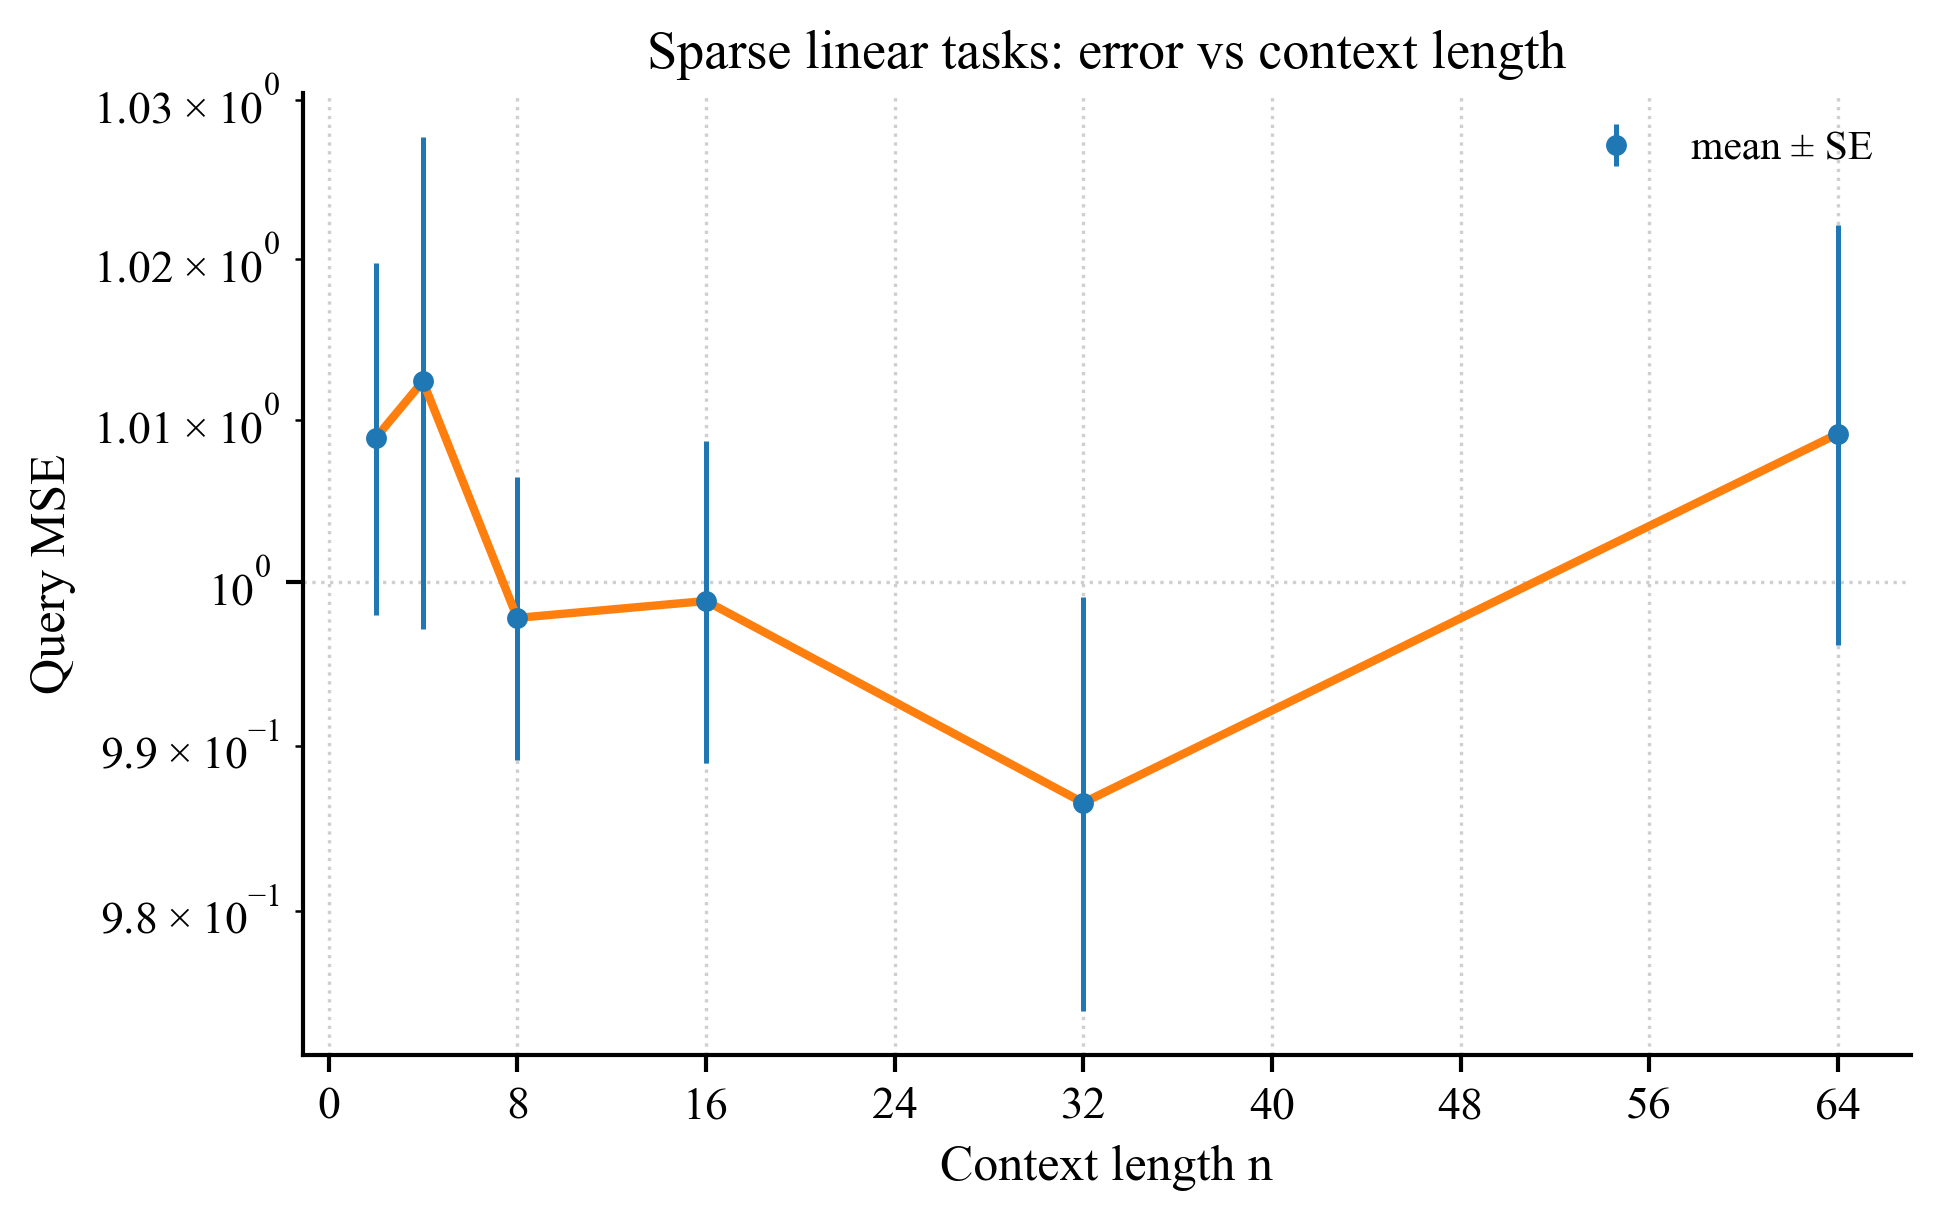
\includegraphics[width=0.8\linewidth]{figures/placeholder.png}
%		\caption{Ablation studies showing the impact of removing attention or MLP components, and using different activation functions. Error bars show standard error over 5 random seeds.}
%		\label{fig:ablation}
%	\end{figure}
%	
%	We conduct ablation studies to verify the necessity of each architectural component and the role of nonlinearity.
%	
%	\paragraph{Component Ablation.}
%	We train three variants:
%	\begin{enumerate}
%		\item \textbf{Full Model:} Standard transformer with attention and MLP.
%		\item \textbf{No Attention:} Replace attention with an identity connection.
%		\item \textbf{Linear MLP:} Replace ReLU MLP with a linear projection.
%	\end{enumerate}
%	
%	\paragraph{Results (\Cref{fig:ablation}, left panel):}
%	\begin{itemize}
%		\item Removing attention increases error by 30-50\%, especially harming performance on tasks requiring similarity matching (RBF).
%		\item Using a linear MLP causes catastrophic failure on nonlinear tasks (Poly, RBF), with errors 3-5× higher, confirming that nonlinearity in the MLP is essential for nonlinear ICL.
%		\item On purely linear tasks, all variants perform similarly, connecting back to prior linear ICL theory.
%	\end{itemize}
%	
%	\paragraph{Activation Function Study.}
%	We test ReLU, GeLU, and Swish activations in the MLP. Results (\Cref{fig:ablation}, right panel) show:
%	\begin{itemize}
%		\item All nonlinear activations perform similarly, with GeLU slightly outperforming others on harder tasks.
%		\item The key factor is \textit{nonlinearity itself}, not the specific activation shape, supporting our theory's reliance mainly on the Lipschitz constant rather than exact form.
%	\end{itemize}
%	
%	\subsection{Summary of Empirical Findings}
%	\label{subsec:empirical_summary}
%	
%	Our experiments provide strong validation for our theoretical framework:
%	\begin{enumerate}
%		\item \textbf{Kernel Equivalence Holds:} Finite-width transformers with SGD behave similarly to kernel ridge regression with the predicted \(K_{\text{total}}\).
%		\item \textbf{Bounds are Predictive:} The \(1/\sqrt{n}\) scaling from our generalization bound accurately describes empirical error decay across diverse tasks.
%		\item \textbf{Phase Transition is Real:} We observe a clear shift in solution sparsity at a critical context length \(n_c\), which scales with task complexity as predicted.
%		\item \textbf{Components are Necessary:} Both attention and nonlinear MLP are essential for nonlinear ICL; neither can be removed without significant performance loss.
%	\end{enumerate}
%	
%	These experiments confirm that our theory captures essential aspects of nonlinear in-context learning, providing not just mathematical guarantees but also practical insights into transformer behavior.
